\documentclass{article}
\pdfpagewidth=8.5in
\pdfpageheight=11in
% The file ijcai21.sty is NOT the same than previous years'
\usepackage{ijcai21}
\usepackage{times}
\usepackage{soul}
\usepackage[hidelinks,hypertexnames=false]{hyperref}
\usepackage{amsthm}

%%% Load required packages here (note that many are included already).
%Permits to copy eg x ⪰ y ⇔ v(x) ≥ v(y) from PDF to unicode data, and to search. From pdfTeX users manual. See https://tex.stackexchange.com/posts/comments/1203887.
	\input glyphtounicode
	\pdfgentounicode=1
%Latin Modern has more glyphs than Computer Modern, such as diacritical characters. fntguide commands to load the font before fontenc, to prevent default loading of cmr.
	\usepackage{natbib}
	\newcommand\hmmax{0}
	\newcommand\bmmax{0}
	\usepackage{lmodern} 
%Encode resulting accented characters correctly in resulting PDF, permits copy from PDF.
	\usepackage[T1]{fontenc}
%UTF8 seems to be the default in recent TeX installations, but not all, see https://tex.stackexchange.com/a/370280.
	\usepackage[utf8]{inputenc}
%	\usepackage{amsmath}
	\usepackage{siunitx}
%Provides \newunicodechar for easy definition of supplementary UTF8 characters such as → or ≤ for use in source code.
	\usepackage{newunicodechar}
%Text Companion fonts, much used together with CM-like fonts. Provides \texteuro and commands for text mode characters such as \textminus, \textrightarrow, \textlbrackdbl.
	\usepackage{textcomp}
%St Mary’s Road symbol font, used for ⟦ = \llbracket.
%	\usepackage{stmaryrd}
\usepackage{centernot}
%Solves bug in lmodern, https://tex.stackexchange.com/a/261188; probably useful only for unusually big font sizes; and probably better to use exscale instead. Note that the authors of exscale write against this trick.
	%\DeclareFontShape{OMX}{cmex}{m}{n}{
		%<-7.5> cmex7
		%<7.5-8.5> cmex8
		%<8.5-9.5> cmex9
		%<9.5-> cmex10
	%}{}
	%\SetSymbolFont{largesymbols}{normal}{OMX}{cmex}{m}{n}
%More symbols (such as \sum) available in bold version, see https://github.com/latex3/latex2e/issues/71.
	\DeclareFontShape{OMX}{cmex}{bx}{n}{%
	   <->sfixed*cmexb10%
	   }{}
	\SetSymbolFont{largesymbols}{bold}{OMX}{cmex}{bx}{n}
%For small caps also in italics, see https://tex.stackexchange.com/questions/32942/italic-shape-needed-in-small-caps-fonts, https://tex.stackexchange.com/questions/284338/italic-small-caps-not-working.
	\usepackage{slantsc}
	\AtBeginDocument{%
		%“Since nearly no font family will contain real italic small caps variants, the best approach is to substitute them by slanted variants.” -- slantsc doc
		%\DeclareFontShape{T1}{lmr}{m}{scit}{<->ssub*lmr/m/scsl}{}%
		%There’s no bold small caps in Latin Modern, we switch to Computer Modern for bold small caps, see https://tex.stackexchange.com/a/22241
		%\DeclareFontShape{T1}{lmr}{bx}{sc}{<->ssub*cmr/bx/sc}{}%
		%\DeclareFontShape{T1}{lmr}{bx}{scit}{<->ssub*cmr/bx/scsl}{}%
	}
%Warn about missing characters.
	\tracinglostchars=2
%Nicer tables: provides \toprule, \midrule, \bottomrule.
	%\usepackage{booktabs}
%For new column type X which stretches; can be used together with booktabs, see https://tex.stackexchange.com/a/97137. “tabularx modifies the widths of the columns, whereas tabular* modifies the widths of the inter-column spaces.” Loads array.
	%\usepackage{tabularx}
%math-mode version of "l" column type. Requires \usepackage{array}.
	%\usepackage{array}
	%\newcolumntype{L}{>{$}l<{$}}
%Provides \xpretocmd and loads etoolbox which provides \apptocmd, \patchcmd, \newtoggle… Also loads xparse, which provides \NewDocumentCommand and similar commands intended as replacement of \newcommand in LaTeX3 for defining commands (see https://tex.stackexchange.com/q/98152 and https://github.com/latex3/latex2e/issues/89).
	\usepackage{xpatch}
%ntheorem doc says: “empheq provides an enhanced vertical placement of the endmarks”; must be loaded before ntheorem. Loads the mathtools package, which loads and fixes some bugs in amsmath and provides \DeclarePairedDelimiter. amsmath is considered a basic, mandatory package nowadays (Grätzer, More Math Into LaTeX).
	\usepackage[ntheorem]{empheq}
%Package frenchb asks to load natbib before babel-french. Package hyperref asks to load natbib before hyperref.
	


\newtoggle{LCpres}
	\newtoggle{LCart}
	\newtoggle{LCposter}
	\makeatletter
	\@ifclassloaded{beamer}{
		\toggletrue{LCpres}
		\togglefalse{LCart}
		\togglefalse{LCposter}
		\wlog{Presentation mode}
	}{
		\@ifclassloaded{tikzposter}{
			\toggletrue{LCposter}
			\togglefalse{LCpres}
			\togglefalse{LCart}
			\wlog{Poster mode}
		}{
			\toggletrue{LCart}
			\togglefalse{LCpres}
			\togglefalse{LCposter}
			\wlog{Article mode}
		}
	}
	\makeatother%

%Language options ([french, english]) should be on the document level (last is main); except with tikzposter: put [french, english] options next to \usepackage{babel} to avoid warning. beamer uses the \translate command for the appendix: omitting babel results in a warning, see https://github.com/josephwright/beamer/issues/449. Babel also seems required for \refname.
	\iftoggle{LCpres}{
		\usepackage{babel}
	}{
	}
	%\frenchbsetup{AutoSpacePunctuation=false}
%listings (1.7) does not allow multi-byte encodings. listingsutf8 works around this only for characters that can be represented in a known one-byte encoding and only for \lstinputlisting. Other workarounds: use literate mechanism; or escape to LaTeX (but breaks alignment).
	%\usepackage{listings}
	%\lstset{tabsize=2, basicstyle=\ttfamily, escapechar=§, literate={é}{{\'e}}1}
%I favor acro over acronym because the former is more recently updated (2018 VS 2015 at time of writing); has a longer user manual (about 40 pages VS 6 pages if not counting the example and implementation parts); has a command for capitalization; and acronym suffers a nasty bug when ac used in section, see https://tex.stackexchange.com/q/103483 (though this might be the fault of the silence package and might be solved in more recent versions, I do not know) and from a bug when used with cleveref, see https://tex.stackexchange.com/q/71364. However, loading it makes compilation time (one pass on this template) go from 0.6 to 1.4 seconds, see https://bitbucket.org/cgnieder/acro/issues/115. Option short-format not usable in the package options as it is fragile, see https://tex.stackexchange.com/q/466882.
	%\usepackage[single]{acro}
	%\acsetup{short-format = {\scshape}}
	%\DeclareAcronym{AMCD}{short=AMCD, long={Aide Multicritère à la Décision}}
\DeclareAcronym{AHP}{short=AHP, long={Analytic Hierarchy Process}}
\DeclareAcronym{AR}{short=AR, long={Argumentative Recommender}}
\DeclareAcronym{DA}{short=DA, long={Decision Analysis}}
\DeclareAcronym{DJ}{short=DJ, long={Deliberated Judgment}}
\DeclareAcronym{DM}{short=DM, long={Decision Maker}}
\DeclareAcronym{DP}{short=DP, long={Deliberated Preference}}
\DeclareAcronym{MAVT}{short=MAVT, long={Multiple Attribute Value Theory}}
\DeclareAcronym{MCDA}{short=MCDA, long={Multicriteria Decision Aid}}
\DeclareAcronym{MIP}{short=MIP, long={Mixed Integer Program}}
\DeclareAcronym{SEU}{short=SEU, long={Subjective Expected Utility}}


\iftoggle{LCpres}{
	%I favor fmtcount over nth because it is loaded by datetime anyway; and fmtcount warns about possible conflicts when loaded after nth.
	\usepackage{fmtcount}
	%For nice input of date of presentation. Must be loaded after the babel package. Has possible problems with srcletter: https://golatex.de/verwendung-von-babel-und-datetime-in-scrlttr2-schlaegt-fehlt-t14779.html.
	\usepackage[nodayofweek]{datetime}
}{
}
%For presentations, Beamer implicitely uses the pdfusetitle option. ntheorem doc says to load hyperref “before the first use of \newtheorem”. autonum doc mandates option hypertexnames=false. I want to highlight links only if necessary for the reader to recognize it as a link, to reduce distraction. In presentations, this is already taken care of by beamer (https://tex.stackexchange.com/a/262014). If using colorlinks=true in a presentation, see https://tex.stackexchange.com/q/203056. Crashes the first compilation with tikzposter, just compile again and the problem disappears, see https://tex.stackexchange.com/q/254257.
%\makeatletter
%\iftoggle{LCpres}{
%	\usepackage{hyperref}
%}{
%	\usepackage[hypertexnames=false, pdfusetitle, linkbordercolor={1 1 1}, citebordercolor={1 1 1}, urlbordercolor={1 1 1}]{hyperref}
%	%https://tex.stackexchange.com/a/466235
%	\pdfstringdefDisableCommands{%
%		\let\thanks\@gobble
%	}
%}
%\makeatother
%urlbordercolor is used both for \url and \doi, which I think shouldn’t be colored, and for \href, thus might want to color manually when required. Requires xcolor.
	\NewDocumentCommand{\hrefblue}{mm}{\textcolor{blue}{\href{#1}{#2}}}
%hyperref doc says: “Package bookmark replaces hyperref’s bookmark organization by a new algorithm (...) Therefore I recommend using this package”.
	\usepackage{bookmark}
%Need to invoke hyperref explicitly to link to line numbers: \hyperlink{lintarget:mylinelabel}{\ref*{lin:mylinelabel}}, with \ref* to disable automatic link. Also see https://tex.stackexchange.com/q/428656 for referencing lines from another document.
	%\usepackage{lineno}
	%\NewDocumentCommand{\llabel}{m}{\hypertarget{lintarget:#1}{}\linelabel{lin:#1}}
	%\setlength\linenumbersep{9mm}
%For complex authors blocks. Seems like authblk wants to be later than hyperref, but sooner than silence. See https://tex.stackexchange.com/q/475513 for the patch to hyperref pdfauthor.
%	\ExplSyntaxOn
%	\seq_new:N \g_oc_hrauthor_seq
%	\NewDocumentCommand{\addhrauthor}{m}{
%		\seq_gput_right:Nn \g_oc_hrauthor_seq { #1 }
%	}
%	%Should be \NewExpandableDocumentCommand, but this is not yet provided by my version of xparse
%	\DeclareExpandableDocumentCommand{\hrauthor}{}{
%		\seq_use:Nn \g_oc_hrauthor_seq {,~}
%	}
%	\ExplSyntaxOff
%	{
%		\catcode`#=11\relax
%		\gdef\fixauthor{\xpretocmd{\author}{\addhrauthor{#2}}{}{}}%
%	}
%	\iftoggle{LCart}{
%		\usepackage{authblk}
%		\renewcommand\Affilfont{\small}
%		\fixauthor
%		\AtBeginDocument{
%		    \hypersetup{pdfauthor={\hrauthor}}
%		}
%	}{
%	}
%I do not use floatrow, because it requires an ugly hack for proper functioning with KOMA script (see scrhack doc). Instead, the following command centers all floats (using \centering, as the center environment adds space, http://texblog.net/latex-archive/layout/center-centering/), and I manually place my table captions above and figure captions below their contents (https://tex.stackexchange.com/a/3253).
	\makeatletter
	\g@addto@macro\@floatboxreset\centering
	\makeatother
%Permits to customize enumeration display and references
	%\nottoggle{LCpres}{
		\usepackage{enumitem} %follow list environments by a string to customize enumeration, example: \begin{description}[itemindent=8em, labelwidth=!] or \begin{enumerate}[label=({\roman*}), ref={\roman*}].
	%}{
	%}
%Provides \Cen­ter­ing, \RaggedLeft, and \RaggedRight and en­vi­ron­ments Cen­ter, FlushLeft, and FlushRight, which al­low hy­phen­ation. With tikzposter, seems to cause 1=1 to be printed in the middle of the poster.
	%\usepackage{ragged2e}
%To typeset units by closely following the “official” rules.
	%\usepackage[strict]{siunitx}
%Turns the doi provided by some bibliography styles into URLs. However, uses old-style dx.doi url (see 3.8 DOI system Proxy Server technical details, “Users may resolve DOI names that are structured to use the DOI system Proxy Server (https://doi.org (current, preferred) or earlier syntax http://dx.doi.org).”, https://www.doi.org/doi_handbook/3_Resolution.html). The patch solves this.
	\usepackage{doi}
	\makeatletter
	\patchcmd{\@doi}{http://dx.doi.org}{https://doi.org}{}{}
	\makeatother
%Makes sure upper case greek letters are italic as well.
	\usepackage{fixmath}
%Provides \mathbb; obsoletes latexsym (see http://tug.ctan.org/macros/latex/base/latexsym.dtx). Relatedly, \usepackage{eucal} to change the mathcal font and \usepackage[mathscr]{eucal} (apparently equivalent to \usepackage[mathscr]{euscript}) to supplement \mathcal with \mathscr. This last option is not very useful as both fonts are similar, and the intent of the authors of eucal was to provide a replacement to mathcal (see doc euscript). Also provides \mathfrak for supplementary letters.
	\usepackage{amsfonts}
%Provides a beautiful (IMHO) \mathscr and really different than \mathcal, for supplementary uppercase letters. But there is no bold version. Alternative: mathrsfs (more slanted), but when used with tikzposter, it warns about size substitution, see https://tex.stackexchange.com/q/495167.
%	\usepackage[scr]{rsfso}
%Multiple means to produce bold math: \mathbf, \boldmath (defined to be \mathversion{bold}, see fntguide), \pmb, \boldsymbol (all legacy, from LaTeX base and AMS), \bm (the most recommended one), \mathbold from package fixmath (I don’t see its advantage over \boldsymbol).
%“The \boldsymbol command is obtained preferably by using the bm package, which provides a newer, more powerful version than the one provided by the amsmath package. Generally speaking, it is ill-advised to apply \boldsymbol to more than one symbol at a time.” — AMS Short math guide. “If no bold font appears to be available for a particular symbol, \bm will use ‘poor man’s bold’” — bm. It is “best to load the package after any packages that define new symbol fonts” – bm. bm defines \boldsymbol as synonym to \bm. \boldmath accesses the correct font if it exists; it is used by \bm when appropriate. See https://tex.stackexchange.com/a/10643 and https://github.com/latex3/latex2e/issues/71 for some difficulties with \bm.
	\usepackage{bm}
	\nottoggle{LCpres}{
	%https://ctan.org/pkg/amsmath recommends ntheorem, which supersedes amsthm, which corrects the spacing of proclamations and allows for theoremstyle. Option standard loads amssymb and latexsym. Must be loaded after amsmath (from ntheorem doc). From cleveref doc, “ntheorem is fully supported and even recommended”; says to load cleveref after ntheorem. When used with tikzposter, warns about size substitution for the lasy (latexsym) font when using \url, because ntheorem loads latexsym; relatedly (but not directly related to ntheorem), size substitution warning with the cmex font happens when loading amsmath and using \url.
%		\usepackage[thmmarks, amsmath, standard, hyperref]{ntheorem}
%		%empheq doc says to do this after loading ntheorem
%		\usetagform{default}
	%Provides \cref. Unfortunately, cref fails when the language is French and referring to a label whose name contains a colon (https://tex.stackexchange.com/q/83798). Use \cref{sec\string:intro} to work around this. cleveref should go “laster” than hyperref.
		\usepackage[capitalise]{cleveref}
	}{
	}
	\nottoggle{LCposter}{
	%Equations get numbers iff they are referenced. Loading order should be “amsmath → hyperref → cleveref → autonum”, according to autonum doc. Use this in preference to the showonlyrefs option from mathtools, see https://tex.stackexchange.com/q/459918 and autonum doc. See https://tex.stackexchange.com/a/285953 for the etex line. Incompatible with my version of tikzposter (produces “! Improper \prevdepth”).
		\expandafter\def\csname ver@etex.sty\endcsname{3000/12/31}\let\globcount\newcount
		\usepackage{autonum}
	}{
	}
%Also loaded by tikz.
	\usepackage{xcolor}
\iftoggle{LCpres}{
	\usepackage{tikz}
	%\usetikzlibrary{babel, matrix, fit, plotmarks, calc, trees, shapes.geometric, positioning, plothandlers, arrows, shapes.multipart}
}{
}
%Vizualization, on top of TikZ
	%\usepackage{pgfplots}
	%\pgfplotsset{compat=1.14}
\usepackage{graphicx}
	\graphicspath{{graphics/}}

%Provides \print­length{length}, useful for debugging.
	%\usepackage{printlen}
	%\uselengthunit{mm}

\iftoggle{LCpres}{
	\usepackage{appendixnumberbeamer}
	%I have yet to see anyone actually use these navigation symbols; let’s disable them
	\setbeamertemplate{navigation symbols}{} 
	\usepackage{preamble/beamerthemeParisFrance}
	\setcounter{tocdepth}{10}
}{
}

%Do not use the displaymath environment: use equation. Do not use the eqnarray or eqnarray* environments: use align(*). This improves spacing. (See l2tabu or amsldoc.)


\newunicodechar{⇒}{\Rightarrow}
\newunicodechar{≠}{\ensuremath{\neq}}
\newunicodechar{≤}{\leq}
\newunicodechar{≥}{\geq}
%… Horizontal Ellipsis
\DeclareUnicodeCharacter{2026}{\ifmmode\dots\else\textellipsis\fi}
\newunicodechar{∧}{\land}
\newunicodechar{∨}{\lor}
\newunicodechar{∩}{\cap}
\newunicodechar{∪}{\cup}
%¬ Not Sign
\DeclareUnicodeCharacter{00AC}{\ifmmode\lnot\else\textlnot\fi}
\newunicodechar{⇔}{\Leftrightarrow}
\newcommand{\N}{ℕ}
\newunicodechar{ℕ}{\mathbb{N}}

\newcommand{\pref}{\succ}%real, connected pref, strict
\newcommand{\prefeq}{\succeq}%real, connected pref, strict
\newcommand{\prefr}{{\succ}^\text{r}}%real, connected pref, strict
\newcommand{\pprefeq}{\succeq^\text{p}}%partial pref
\newcommand{\ppref}{\succ^\text{p}}%partial pref
\newcommand{\pprefinv}{\prec^\text{p}}%partial pref
\newcommand{\nppref}{\nsucc^\text{p}}%negated partial pref
\newcommand{\linors}{\mathcal{L}(A)}
%https://tex.stackexchange.com/a/45732, works within both \set and \set*, same spacing than \mid (https://tex.stackexchange.com/a/52905).
\newcommand{\suchthat}{\;\ifnum\currentgrouptype=16 \middle\fi|\;}

%Thanks to https://tex.stackexchange.com/q/154549
\makeatletter
\newcommand{\newrelation}[2]{% #1 = control sequence, #2 = replacement text
	\@ifdefinable{#1}{%
		\def#1{%
			\@ifnextchar_{\csname\string#1\endcsname}{\mathrel{#2}}%
		}%
		\@namedef{\string#1}##1##2{\mathrel{#2_{##2}}}%
	}%
}
\makeatother

\newrelation{\prefinc}{\!\parallel\!}%partial pref, complement (incomparable)
\newrelation{\pinc}{\bowtie^\text{p}}
%\newrelation{\prefinc}{Q^\text{p}}%partial pref, complement (incomparable)

\newcommand{\profile}{\bm{v}}%(complete) profile
\newcommand{\pprofile}{{\bm{p}}}%partial profile
\newcommand{\w}{\bm{w}}
\newcommand{\W}{\mathcal{W}}
\newcommand{\Co}{\mathcal{C}}
\newcommand{\pw}{W}%our knowledge about the weights
\newcommand{\powersetz}[1]{\mathscr{P}^*(#1)}
\newcommand{\strat}[1]{\emph{#1}}

\newcommand{\intvl}[1]{\llbracket #1 \rrbracket}

\DeclareMathOperator{\Regret}{Regret}
\DeclareMathOperator{\SCORE}{Score}
\DeclareMathOperator{\PMR}{PMR}
\DeclareMathOperator{\MaxR}{MR}
\DeclareMathOperator{\MMR}{MMR}
\DeclareMathOperator{\leximax}{leximax}
\DeclareMathOperator*{\argmax}{argmax}
\DeclareMathOperator*{\argmin}{argmin}

\DeclareMathDelimiter{(}{\mathopen} {operators}{"28}{largesymbols}{"00}
\DeclareMathDelimiter{)}{\mathclose}{operators}{"29}{largesymbols}{"01}

\newtheorem{claim}{Claim}
\newtheorem{prop}{Proposition}
\newtheorem{corollary}{Corollary}
\newtheorem{definition}{Definition}
\newtheorem{example}{Example}

\DeclarePairedDelimiter\set{\{}{\}}
\DeclarePairedDelimiter\card{\lvert}{\rvert}
\DeclarePairedDelimiter\abs{\lvert}{\rvert}

\newtheorem{proof}{Proof}
%for appendix
\usepackage{import}
\usepackage{algorithm, algpseudocode}
\usepackage{booktabs}
\usepackage{pgfplots}
\pgfplotsset{compat=1.16}

\setlist[itemize]{noitemsep, topsep=0pt}

\newcommand{\commentOC}[1]{\textcolor{blue}{\small$\big[$OC: #1$\big]$}}
\newcommand{\commentBN}[1]{\textcolor{red}{\small$\big[$BN: #1$\big]$}}

\pdfinfo{
	/TemplateVersion (IJCAI.2021.0)
}

%I find these settings useful in draft mode. Should be removed for final versions.
	%Which line breaks are chosen: accept worse lines, therefore reducing risk of overfull lines. Default = 200.
		\tolerance=2000
	%Accept overfull hbox up to...
		\hfuzz=2cm
	%Reduces verbosity about the bad line breaks. TODO reduce
		\hbadness 10000
	%Reduces verbosity about the underful vboxes.
		\vbadness=6000

%%% Use this command to specify the title of your paper.

\title{Simultaneous Elicitation of Scoring Rule and Agent Preferences for Robust Winner Determination}

%%% Provide names, affiliations, and email addresses for all authors.

\author{ID: 3177}

%\author{
%	Beatrice Napolitano$^1$\footnote{Contact Author}\and
%	Olivier Cailloux$^1$\and
%	Paolo Viappiani$^2$\\
%	\affiliations
%	$^1$Université Paris-Dauphine, Université PSL, CNRS, LAMSADE\\
%	$^2$LIP6, UMR 7606, CNRS and Sorbonne Universit\'e\\
%	\emails
%	\{beatrice.napolitano, olivier.cailloux\}@dauphine.fr,
%	paolo.viappiani@lip6.fr
%}

         
\newcommand{\BibTeX}{\rm B\kern-.05em{\sc i\kern-.025em b}\kern-.08em\TeX}

%%%%%%%%%%%%%%%%%%%%%%%%%%%%%%%%%%%%%%%%%%%%%%%%%%%%%%%%%%%%%%%%%%%%%%%%

\begin{document}

\maketitle 

\begin{abstract}
Social choice deals with the problem of determining a consensus choice from the preferences of different agents.
In the classical setting, the voting rule is fixed beforehand and full information concerning the preferences of the agents is provided.
This assumption of full preference information has recently been questioned by a number of researchers and
	several methods for eliciting the preferences of the agents have been proposed.
	%  are completely known have been proposed, as well as techniques that consider the opposite scenario. 

In this paper we argue that in many situations one should consider as well the voting rule to be 	partially specified.
%	This article goes one step further by tackling one important new case, namely, when both the voting rule and the agents preferences are partially known. It also permits to obtain a progressively refined recommendation without requiring to achieve full knowledge of either sort of information.
%This is useful because providing such information is often costly: the chair may find it hard to specify a rule completely; agents may need time to form reflective preferences.	
	Focusing on positional scoring rules, we assume that the chair, while not able to give a precise definition of the rule, is capable of answering simple questions requiring to pick a winner from a concrete profile. In addition, we assume that the agent preferences also have to be elicited. %and are acquired by asking comparison queries. 
	We propose a method for robust approximate winner determination and interactive elicitation based on minimax regret; we develop several strategies for choosing the questions to ask to  the chair and the agents in order to %acquire the most relevant information for
converge quickly to a near-optimal alternative. Finally, we analyze these strategies in experiments %in order to validate our approach
 %focusing on settings 
 where the  rule and the preferences are simultaneously elicited.
 %and obtain practical guidelines.
\end{abstract}

\section{Introduction}
Aggregation of preference information is a central task in many computer systems (recommender systems, search engines, etc).
In many situations, such as in group recommender systems, the goal is to find a consensus choice;
social choice theory can provide foundations for such applications

%The traditional approach to social choice assumes that both the social choice function and the full preference orderings of the agents (voters) are expressed beforehand. These represent two strong hypothesis.
The traditional approach to social choice assumes that 1) the social choice function and 2) the full preference orderings of the agents are expressed beforehand. These represent two strong hypothesis.

Requiring agents to express full preference orderings can be prohibitively costly (in terms of cognitive and communication cost).
This observation has motivated several works assuming partial preference orders; 
%and incremental elicitation of agent preferences. 
%In the context of social choice, several authors have been interested in obtaining information about winners with reduced assumptions about the knowledge of the agent preferences (assuming that the voting rule is known).
one early work is  by \Citet{Conitzer2005} who studied the complexity of communication when using different voting rules. %determining lower and upper bounds;
%they showed that, 
%in the worst case, the agents should send their complete set of preference for several rules. 
\Citet{Konczak05} studied the computation of possible and necessary winners for various voting rules; %and showed that the problem is hard in the general case.
\citet{Xia2008} then showed that, while the identification of a necessary co-winner in scoring rules is polynomial,  the determination of possible co-winners is NP-hard;
% they also  proposed polynomial-time algorithms when using maximin and Bucklin.
additional complexity results were given by \citet{Walsh2007} and \citet{Pini2007}.
%\citep{Walsh2007} showed that the general case remains computationally hard even when restricting to single-peaked preferences;  sufficient conditions that ensure tractability were then found \citep{Pini2007}.

Since in many practical situations there would be too many possible winners but no necessary winners,  
several works addressed the problem of  elicitation of agent preferences \citep{Naamani-Dery2015,Kalech2011,Lu2011,Pini2009,Benabbou2016,Dey2016,Dey2016_2}  using a variety of approaches (minimax regret, Bayesian methods, etc.) with the goal of converging to a necessary winner; \citep{Walsh2009,Conitzer2009}  analyzed when to stop the elicitation process.

Furthermore, it is often difficult for non-experts to formalize a voting rule on the basis of some generic preferences over a desired aggregation method. Thus, the first hypothesis should also be relaxed. 
%While most of the focus in the research community has been in dealing with incomplete agent preferences, 
Consider, as an example, a committee that is about to hire a new employee, whose performances are evaluated by several experts. The members of the committee may not have a voting rule in mind at the start of the process, and might not wish to agree on a specific voting rule, but they might be willing to answer a few questions requiring to select who should be the winner out of specific profiles. 
%The information provided can be used to   % to determine their employee of choice.

%This paper considers both sources of uncertainty at the same time, and proposes a method able to recommend a consensus choice without requiring full knowledge of either.
In this paper we focus on positional scoring rules, that are a particularly common method used to aggregate rankings. 
We develop methods, based on the notion of minimax regret, for determining a robust ``winner'' under uncertainty of both the voting rule and the agent preferences.
%alternative using positional scoring rules and 
We provide incremental elicitation methods that 
at each step of the elicitation ask a question either to one of the agents or to the chair (the person or organization supervising the voting process) and discuss several heuristics that determine queries that quickly reduce regret. 
Answers to questions are encoded in terms of constraints; questions to the agents are comparisons between pairs of alternatives while
questions to the chair ask  to select who should be the winner in a synthetic profile.

While some previous works have considered partially specified aggregation methods \citep{Stein1994,Llamazares2013,Viappiani2018}, we do not know of any work considering both sources of uncertainty at the same time. 
%has dealt with %scenarios where it is instead the voting rule that is partially defined. % but the preferences are given. 
%a  partially defined voting rule.
%While previous works have considered either partial information about the agent preferences or a partially specified aggregation method, we do not know of any work considering both sources of uncertainty at the same time.
Actually, very few works altogether have considered the problem of eliciting a voting rule by asking questions to the chair;  we are aware of the work of \Citet{Cailloux2014}, that assumes a different representation for the rule. %we mention the work of \Citet{Cailloux2014} considering elicitation the voting rule by assuming a specific representation.

%A classic paper is the one by \citet{Stein1994} that, considering scoring rules, identified dominance relations between alternatives; these relations allow to determine pairs of alternatives where the first is at least as good as the second no matter which weights are chosen among a generic class of weights (decreasing weighs or convex decreasing weights).
%More recent articles considered the problem of dealing with unspecified weights in positional scoring rules: \citet{Llamazares2013} proposed a method based on Data Envelopment Analysis (DEA), while \citet{Viappiani2018} proposed to aggregate the uncertainty in weights using criteria used in decision-making under uncertainty (such as minimax regret). 
% provided an elicitation framework for a different class of rules.

Let us also mention works addressing the manipulability of voting rules \citep{Elkind2012,Dey2018,Dey2018_2,Conitzer2011,Baumeister2019}, and studies of strategic behaviors
% when agents learn incrementally about other agent preferences
 \citep{Endriss2016,Lev2019,Annemieke2012}.

Our approach is evaluated in simulations where both the voting rule and the agent's preferences are initially unknown to the system and incrementally revealed by answering questions.
We compare the effectiveness of several strategies of choosing questions depending on the current knowledge.
In this work:
\begin{itemize}
	\item we provide a novel mechanism for elicitating a voting rule by translating abstract questions about weights to direct choice questions about a profile;  
	\item we show that in small problem sizes, starting with zero knowledge, it is possible to reach a low regret level with a reasonable number of questions;
	\item we present elicitation strategies that achieve good results within reasonable computation time for small problem sizes;
	\item we show that for the class of rule considered, asking a few questions about the voting rule suffice to reach a low regret level;
	\item our experiments suggest that low degree of similarity among preference rankings (like in the case of impartial culture) is a more challenging setting than less varied profiles.
\end{itemize}

\section{Social choice with partial information}
\label{sec:background}
We now introduce some basic concepts.
We consider a set $A$ of $m$ alternatives (products, restaurants, public projects, job candidates, etc.), an infinite set $\N$ of potential agents and a specific finite set of agents $N^* \subset \N$.

A {\em profile} $(\pref_j, j \in N)$ considers a finite subset of agents $N \subset \N$ and associates to each agent a preference order ${\pref_j}  \in \linors$, a linear order over the alternatives.
A profile is equivalently represented by $\profile=(v_j, j \in N)$ where $v_j(x) \in \set{1, \ldots, m}$ denotes the rank of alternative $x$ in the preference order $\pref_j$. 
A social choice function $f : \cup_{\emptyset ≠ N \subset \N} \linors^N \rightarrow \powersetz{A}$ associates to each profile a set of (tied) winners, where $\powersetz{A}$ represents the set of subsets of $A$ except for the empty set.
Among the many possible social choice functions, we consider convex {\em positional scoring rules (PSRs)}. A PSR $f^{\w}$ is parameterized by a \emph{scoring vector} $\w$ associating weights $w_r \in [0, 1]$ to positions, with $1 = w_1 ≥ w_2 ≥ … ≥ w_m = 0$.
Let $\alpha^{x}_r$ be the number of times that alternative $x$ was ranked in the $r$-th position.
Given $\profile$ and $\w$, an alternative $x \in A$ obtains the score
\begin{align}
	\label{eq:srule}
	s(x; \profile, \w) = \sum_{j=1}^{n} w_{v_j(x)}
	= \sum_{r=1}^{m} \alpha^{x}_r w_r\ .
\end{align}
The winners $f^{\w}(\profile)$ are the alternatives with highest score.

An important class of PSRs is the one using convex weights \citep{Stein1994,Llamazares2016}, meaning that the difference between the weight of the first position and the weight of the second position is at least as large as the difference between the weights of the second and third positions, etc.
\begin{equation} 
	\label{eq:convexity}
	\forall r \in \{1,\ldots,m-2\}: w_r - w_{r+1} \geq w_{r+1}-w_{r+2}.
\end{equation}
The constraint above is a natural and common assumption, often used when aggregating rankings in sport competitions: losing ranks at the top of the ranking is more damaging than losing ranks at the bottom.
Let $\W$ denote the set of such convex weight vectors.

Let $\profile^* = (\pref_j^*, j \in N^*)$ and $\w^*$ denote the profile and weight vector, unknown to us, that represent the preferences of the agents in $N^*$ and of the chair. 

At a given time, our knowledge of agent $j$'s preference is encoded by a partial order ${\ppref_j} \subseteq {\pref_j^*}$ over the alternatives, a transitive and asymmetric relation (we assume that preference information is truthful).
%We use $\prefinc$ to denote incomparability, that is $a \prefinc_{j} b$ iff $a \nppref_j b \wedge b \nppref_j a$.
An incomplete profile $\pprofile = (\ppref_j, j \in N^*)$ maps each agent to a partial preference.
Let $C(\ppref_j) = \set{{\succ} \in \linors \suchthat {\ppref_j} \subseteq {\succ}}$ denote the set of possible completions of $\ppref_i$ and $C(\pprofile) = \prod_{j \in N} C(\ppref_j)$ the set of complete profiles extending $\pprofile$. Note that $\profile^* \in C(\pprofile)$.

The vector $\w^*$  is also unknown but we assume that the chair is able to specify additional preference information taking the form of linear constraints about $\w^*$. Let $\pw \subseteq \W$ denote the set of weight vectors compatible with the preferences expressed by the chair about the scoring vector.
%Of course it may be difficult for real decision makers to state preferences about the voting rule in such an abstract way.
We will show in \cref{sec:elicit} that the additional preferences we use can be elicited by showing a complete profile of a synthetic election and asking who should be elected in this case.

\section{Robust winner determination}
\label{sec:mmr}
It is desirable in an elicitation protocol such as ours to be able to stop before reaching full knowledge of the agent preferences or of the preferences of the chair about the voting rule. As, often, there are no necessary winners and too many possible winners, it is useful to declare a winner given partial information.
As a decision criterion to determine a winner, we propose to use minimax regret \citep{Savage1954}. 
This decision criterion has been used for robust optimization under data uncertainty \citep{Kouvelis1997} as well as in decision-making with uncertain utility values \citep{Salo2001,Boutilier2006}.
In particular, \citet{Lu2011} have adopted minimax regret for winner determination in social choice where
the preferences of agents that are partially known, while the social choice function is known.

We consider the simultaneous presence of incomplete knowledge in agent preferences and in the weights of the PSR.
We use \emph{maximum regret} to quantify the worst-case error, and let the alternatives that minimize this quantity win, giving some robustness in face of ignorance.
Intuitively, the quality of a proposed alternative $a$ is how far $a$ is from the optimal one in the worst case, given the current knowledge.

The maximum regret is considered by assuming that an adversary can both 1) extend the partial profile $\pprofile$ into a complete profile, and 2) instantiate the weights choosing among any weight vector in $\pw$, where $\pprofile$ and $\pw$ represent our knowledge so far.
We formalize the notion of minimax regret in multiple steps.
First of all, $\Regret(x, \profile, \w) = \max_{y \in A} s(y; \profile,\w) - s(x; \profile, \w)$ is the “regret” of selecting $x$ as a winner instead of choosing the optimal alternative under $\profile$ and $\w$.
The pairwise maximum regret $\PMR(x,y;\pprofile,W) = \max_{\w \in W} \max_{\profile \in C(\pprofile)} s(y; \profile,\w) - s(x; \profile,\w)$ of $x$ relative to $y$ given the partial profile $\pprofile$ and the set of weights $W$
is the worst-case loss of choosing $x$ instead of $y$ under all possible realizations of the full profile {\em and} all possible instantiations of the weights.
The maximum regret $\MaxR(x;\pprofile,W) = \max_{y \in A} \PMR(x,y; \pprofile, W) = \max_{\w \in W} \max_{\profile \in C(\profile)} \Regret(x; \profile, \w)$ is the worst-case loss of $x$. That is the loss occurred as the result of an adversarial selection of the complete profile $\profile \in C(\pprofile)$ and of the scoring vector $\w \in W$ that together maximize the loss between $x$ and the true winner under $\profile$ and $\w$.
Finally,  $\MMR(\pprofile,W) = \min_{x \in A} \MaxR(x;\pprofile,W)$ is the value of minimax regret under $\pprofile$ and $W$, obtained when recommending a minimax optimal alternative $x^*_{\pprofile, W} \in A^*_{\pprofile, W} = \argmin_{x \in A} \MaxR(x;\pprofile,W)$.
Picking as consensus choice an alternative associated with minimax regret provides a recommendation that gives worst-case guarantees. 
In cases of ties in minimax regret, we can return all minimax alternatives $A^*_{\pprofile, W}$ as winners or pick one of them using some tie-breaking strategy.

Observe that if $\MMR(\pprofile, W)\!=\!0$, then any $x^{*}_{\pprofile,W} \in A^*_{\pprofile, W}$ is a necessary winner: any valid completion of the profile and choice of $w \in W$ gives to $x^{*}_{\pprofile,W}$ the highest score.

We note that our notion of regret gives some cardinal meaning to the scores: instead of just being used to select winners under the corresponding PSR, their differences are considered as representing the regret of the chair.

% Add some general remarks about using minimax regret

\paragraph{Computation of minimax regret}
Given a voting rule and a partially specified profile, \citet{Xia2008} determine necessary winners by showing constructions that attempt to maximize the score difference between a proposed winner and a chosen alternative. This reasoning was later adopted by \citet{Lu2011} who used the considerations on the worse-case completions for computing the minimax regret. 

In order to compute pairwise maximum regret, and therefore minimax regret, we decompose the PMR into the contributions associated to each agent by adapting this same reasoning to our setting. The context is however more challenging due to the presence of uncertainty in the weights.

Recall that, in the computation of $s(x; \profile, \w)$, $w_{v_j(x)}$ represents the score that $x$ obtains in the ranking $v_j$ (see \cref{eq:srule}).
Since scoring rules are additively decomposable, we can consider separately the contribution of each agent to the total score. Thus, we can write the actual regret of choosing $x$ instead of $y$ as $s(y; \profile,\w) - s(x; \profile, \w) = \sum_{j=1}^n w_{v_j(y)} - w_{v_j(x)}$, and we obtain $\PMR(x,y; \pprofile, W) =  \max_{\w \in W} \sum_{j=1}^{n} \max_{v_j \in C(\succ_j^p)} [w_{v_j(y)} - w_{v_j(x)}]$.
%Note that in general the inner max depends on the weights chosen by the outer max.

The following propositions (with proofs in appendix) show that the procedure for completing a partial profile that was first proposed by \citet{Lu2011} when considering a fixed weight vector also applies in our setting. We write $a \pprefeq_j b$ iff $a \ppref_j b \lor a = b$ and adopt the canonical notation when considering a relation as a function, writing for example ${\pprefeq_j}(x)$ to designate $\set{y \suchthat x \pprefeq_j y}$.

\begin{proposition} \label{claim:completion}
	There exists a completion $\hat{\profile} \in C(\pprofile)$ of the profile $\profile$ such that $\PMR(x,y; \pprofile, W) = \max_{\w \in W} [ s(y; \hat{\profile}, \w) - s(x; \hat{\profile}, \w) ]$ and such that the linear order $\hat{v}_{j}$ of each agent $j$ satisfies:
	\begin{align} 
		\label{eq:complx}
		a \pref_j x &⇔ ¬(x \pprefeq_j a)\\
		\label{eq:comply}
		y \pref_j a &⇔ ¬(a \pprefeq_j y) ∧ ¬((x \pprefeq_j y) ∧ ¬(x \pprefeq_j a)).
	\end{align} 
\end{proposition}

\begin{proposition} \label{claim:rankPMR}
	The rank of $x$ in the PMR-maximizing linear orders of agent $j$ is $\hat{v}_{j}(x) = 1+\card{A}-\card{{\pprefeq_j}(x)}$, and the rank of $y$ is $\hat{v}_{j}(y)=1+\card{{\pprefinv_j}(y)}+\card{\beta}$, where $\card{\beta} = \card{A \setminus ({\pprefeq_j}(x) \cup {\pprefinv_j}(y))}$ if $(x \pprefeq_j y)$ and $\card{\beta} = 0$ otherwise.
\end{proposition}

\begin{proposition}
	The $\PMR$ can be written as:
	\begin{align} 
		\PMR(x,y; \pprofile, W)  
		& = \max_{w \in W} \sum_{j=1}^n w_{\hat{v}_j(y)} - w_{\hat{v}_j(x)} \\ 
		& = \max_{w \in W} \sum_{r=1}^m (\hat{\alpha}_{r}^{y} - \hat{\alpha}_{r}^{x}) w_i. 
	\end{align}
	where $\hat{\alpha}_{r}^{y}$ (resp. $\hat{\alpha}_{r}^{x}$)  is the number of times $y$ (resp. $x$) has rank $r$ in the complete profile $\hat{\profile}$ defined in \cref{claim:rankPMR}. %\ref{claim:completion}.
\end{proposition}

(\cref{claim:rankPMR} can be understood by observing that in the case $(x \pprefeq_j y)$, $\beta$ is the number of alternatives incomparable with both $x$ and $y$.)
The last proposition shows that PMR is linear in the weights.
%Recall that $\pw$ represents the weight vectors compatible with the preferences of the chair stated so far.
The pairwise max regret $\PMR(x,y; \pprofile,W)$ can thus be obtained by solving the following linear program defined on the variables $w_1, …, w_m$:
\begin{align}
	\max_{\w} & \sum_{r=1}^m (\hat{\alpha}_{r}^{y} - \hat{\alpha}_{r}^{x}) w_{r}\\
	\text{ s.t. } & w_1 = 1 ≥ … ≥ w_m = 0, \text{\cref{eq:convexity}} \text{ and } \w \in \pw.
\end{align}
%Note that given our choice $w_{1}=1$ and $w_{m}=0$, there are only $m-2$ variables 
%(we leave $w_{1}$ and $w_{m}$ in the LP just for clarity of presentation).

The max regret $\MaxR(x; \pprofile, W)$ is determined by considering the pairwise regret of $x$ with all other alternatives in $A$, and the recommended alternatives are the ones with least max regret. 
Observe that when the $\PMR$ of an alternative $x$ (against some other alternative $y$) exceeds the best MR value found so far, we do not need to further evaluate $x$. 
This idea can be exploited using a minimax-search tree \citep{Braziunas2012}.

\section{Interactive Elicitation} 
\label{sec:elicit}
We propose an incremental elicitation method based on minimax regret.
At each step, the system may ask a question either to one of the agents about her preferences or to the chair about the voting rule. 
The goal is to obtain relevant information to reduce minimax regret as quickly as possible.
The elicitation can be terminated either after a given number of questions, or when the minimax regret is lower than a threshold (or when it drops to zero if we wish optimality).

%As termination condition of elicitation, we can check whether minimax regret is lower than a threshold; or after having asked a given number of questions.
%if we wish optimality, we can perform elicitation until minimax regret drops to zero.

%The remainder of this section is structured as follows.
%First, we discuss the different types of questions that can be asked to the agents and to the chair, and the way responses are handled.
%Then, we describe different strategies to determine informative queries to ask next, with the goal of reducing $\MMR(\pprofile,W)$ quickly.

\paragraph{Question types}
We distinguish between questions asked to the agents and questions asked to the chair.
As {\em questions asked to the agents} we consider comparison queries relating two alternatives.
%Another common type of queries are {\em top-k}, asking to each agent her $k$ most preferred alternatives.
The effect of a response to a question asked to an agent is the increase in our knowledge about the agent rankings, thus augmenting the partial profile $\pprofile$. 
If agent $j$ answers a comparison query stating that alternative $a$ is preferred to $b$, then the partial order $\ppref_j$ is augmented with $a \ppref_j b$ and by transitive closure.

A bit more discussion is needed about {\em questions asked to the chair}.
Such questions aim at refining our knowledge about the scoring rule; a response gives us a constraint on the weight vector $\w$.
In particular, we want to obtain constraints of the type $w_{r} - w_{r+1} \geq \lambda (w_{r+1} - w_{r+2})$ for $r \in \{1,\ldots,m-2\}$, relating the difference between the importance of ranks $r$ and $r+1$ with the difference between ranks $r+1$ and $r+2$.

\paragraph{Building concrete questions for the chair}
Even if the chair might be considered able to answer directly such abstract questions, we want to ensure that these questions can also, in principle, be asked in a more concrete way: in terms of winners of example profiles. Such questions have precise semantics whose understanding can be assumed to be shared by the chair, contrary to abstract questions about weights. 
Moreover, this way of questioning the chair is independent of the voting rule that is being elicited. Asking questions about weights only works when a scoring rule is being considered.
Asking who should win in specific profiles has been used in experimental settings investigating the feeling of justice of individuals \citep{Giritligil2005}, but, to the best of our knowledge, the use of such questions to systematically guide an elicitation process about voting rules is novel. 
This is similar to favor, in decision theory, direct choice questions ("please choose either a or b") compared to questioning the decision maker about the shape of her utility function. The former are considered “observable”: acts of choice are translated to preference statements \citep{colell_microeconomic_1995}. 

Thus, our task is to build a profile, given $\lambda$ and $r ≤ m-2$, in such a way that the set of (tied) winners picked by the chair reveals whether $w_{r} - w_{r+1} \geq \lambda (w_{r+1} - w_{r+2})$.
\begin{proposition}\label{prop:chairQuestions}
	Given a rational $\lambda = p/q > 1$ and a rank $r$ between $1$ and $m - 2$, there exists a profile $P$ such that, for any weight vector $\w \in \W$, $a \in f(P)$ iff $w_{r} - w_{r+1} ≥ \lambda (w_{r+1} - w_{r+2})$ and $b \in f(P)$ iff $w_{r} - w_{r+1} ≤ \lambda (w_{r+1} - w_{r+2})$, where $f$ is the PSR parameterized with $\w$.
\end{proposition}

\begin{example*}
	Suppose we want to ask the following question to the chair: $w_{2} - w_{3} ≥ 2 (w_{3} - w_{4})$. 
	We then show the following profile to the chair and ask who should win (each column is a preference of a voter).
	\begin{center}
		$
		\begin{array}{ccccccccc}
			c&d&d&a&a&a&b&b&b\\
			a&c&c&b&b&b&a&a&a\\
			b&b&b&c&c&c&d&d&d\\
			d&a&a&d&d&d&c&c&c\\
		\end{array}.
		$
	\end{center}
	Both $a$ and $b$ have scores higher than $c$ and $d$ for all convex weights, thus either $a$ or $b$ will be picked under our hypothesis; and $s(a) ≥ s(b) ⇔ w_2 + 2 w_4 ≥ 3 w_3$.
	(\cref{proof:chairQuestions} presents the general method of constructing such profile.)
\end{example*}

\paragraph{Elicitation strategies}
We develop several strategies for simultaneous elicitation of agent preferences and of the PSR.
While it is of course possible to first fully elicit the agent preferences and afterwards elicit weights, we want to investigate experimentally approaches that are able to recommend winning alternatives before obtaining complete knowledge of the profile or the rule.
%Indeed, it can be beneficial to split efforts asking questions to the chair and to agents, depending on which is estimated to be more informative.
We define here the various strategies we tested experimentally. A strategy tells us, given the current partial knowledge $(\pprofile, W)$, which question to ask next.

The \strat{Random} strategy gives a baseline for comparison and informs about the difficulty of an elicitation problem. 
It first chooses equiprobably whether to question the chair or the agents. In the first case, it draws one rank in $1 ≤ r ≤ m-2$ equiprobably, takes the middle of the interval of values for $\lambda$ that are still possible considering our knowledge so far, and asks whether $w_r - w_{r+1} ≥ \lambda (w_{r+1} - w_{r+2})$.
%The intervals are initialized to $[1, n]$: $\lambda≥1$ by convexity and we assume $\lambda≤n$ wlog, in fact for $\lambda≥n$, the rule coincides with Plurality.
In the second case, it draws equiprobably among the agents whose preference is not known entirely; draws an alternative $a$ equiprobably among those involved in some incomparabilities in $\ppref_j$; and draws an alternative $b$ equiprobably among those incomparable with $a$ in $\ppref_j$.

Let $(x^{*},\bar{y}, \bar{\profile}, \bar{\w})$ be the current solution of the minimax regret, where $x^{*}$ is the minimax optimal alternative and $\bar{y}, \bar{\profile}, \bar{\w}$ the corresponding adversarial choices. 
The \strat{Pessimistic} strategy considers a set of $n + m$ candidate questions: one per agent, and one per rank \commentOC{Isn’t this $m-2$?}.
The candidate questions to the agents are chosen by extending the idea of \citet{Lu2011}, that priviledge learning about the relationship of $x^*$ and $\bar{y}$ to the other alternatives if possible.
The candidate questions to the chair are determined as in the Random strategy.
The Pessimistic strategy selects among these $n + m$ candidate questions one that leads to minimal regret in the worst case: for each question we compute the minimax regret for the two possible answers, considering a penalty terms depending on the kind of question, and choose the best according to (quasi-)$\leximax$. \Cref{sec:appendix} provides more details.

The \strat{Extended pessimistic} strategy uses the same criterion as the pessimistic strategy, but extending it to a bigger set of candidate questions, the same as those considered by the Random strategy. These candidate questions are then evaluated using the same operator as for the Pessimistic strategy.
We use this strategy to test whether Pessimistic performs well: depending on the quality of the heuristic of the Pessimistic strategy, it might perform nearly equally well, or perhaps even better, than Extended pessimistic, while being (much) faster. Extended pessimistic is applicable only to small problem instances: its complexity is in $O(n^2 m^5)$, because we consider $O(m^2)$ questions for each agent and need for each question to compute MMR twice, whose complexity is $O(nm^3)$.

The \strat{Two phases} strategy is developed in order to investigate the effect of varying the proportion of questions asked to agents and to the chair, and compare the performance of asking questions to the chair first or to the agents first. It is parameterized by $q_c$, a value indicating the number of questions that must be asked to the chair.
The \strat{Two phases-ca} variant first asks $q_c$ questions to the chair, then $k - q_c$ questions to the agents, using in both cases Pessimistic to select the specific questions; whereas the \strat{Two phases-ac} variant starts with $k - q_c$ questions to the agents, then questions the chair. 
%Note that when asking first only questions to the chair, if the obtained knowledge approximates well the scoring vector, then in the second part of the elicitation we fall into the more classical setting of incompleteness of preferences assuming a known voting rule. 
%And vice-versa when asking first questions to the agents, the second part of the elicitation is similar to the setting of incompletely specified scoring rule. 
%This strategy also permits to simulate the current state of the art when considering incomplete preferences. By asking enough questions to the chair we can reduce our problem into a well studied one of incompleteness of preferences knowing the voting rule. Similarly, if we invert to whom ask questions first, we fall instead in an already studied case of uncertainty of the voting rule with a known complete profile. 

Finally, the \strat{Elitist} strategy aims at uncovering as quickly as possible the top alternative of each agent. It asks $m - 1$ questions to each agent in turn. 
Given an agent to query $j$, it asks about an alternative currently undominated in $\ppref_j$ and any alternative that is currently incomparable to this alternative. Thus, the top alternative in the ranking of $j$ will be known after having asked exactly $m-1$ questions to $j$.
After having asked $n (m-1)$ questions to the agents, it questions the chair only, using the same approach as the Pessimistic strategy.
This strategy can be expected to perform well when the chair assigns a large weight to the first rank, as compared to the other ranks. It will be useful to further challenge the Pessimistic strategy, which is not specifically tailored to such a situation.

%\item {\em Volumetric} strategy: chooses an agent $i$ and a query that maximizes the number of new pairwise preferences revealed given the worst response.

\section{Empirical Evaluation} 
\label{sec:experiments}
We  performed a number of numerical experiments using both real data and generated profiles in order to validate our approach and test the performance of our elicitation strategies. %Our experiments are described by topic here below. 
%We start by describing the general protocol of experimentation. %use the following protocol, deviations are indicated below for each experiment.

Given a problem size $(m, n)$, a number of questions $k$ and a strategy to test, we first create an “oracle”, representing the true preferences of the agents (randomly generated or coming from real data) and the weights associated with the chair’s scoring rule (randomly generated).
We start with empty knowledge ($\pprofile = \emptyset, W = \W$) about the preference orderings of the agents and the weight differences favored by the chair. We obtain the first question to be asked using the strategy under test. We then use the oracle to answer the question and update the system's knowledge, which is thus used to obtain the next question. This is repeated until $k$ answers have been obtained, computing the resulting MMR values along the way for various values of $k$. We repeat this whole experiment a variable number of times, for a given $(m, n, k)$, and report the average resulting MMR and standard deviation \textit{sd}. The sizes of the considered scenarios are comparable to the ones used by \citet{Cailloux2014}. 

The oracle is built as follows. 
For the real preferences, we used the following data sets from \href{https://www.preflib.org/}{PrefLib} \citep{PrefLib}. \textit{T Shirt}: $m = 11$ tee shirt designs voted by $n = 30$ members of the Optimization Research Group at NICTA; \textit{AGH Course Selection}: $m = 9$ courses evaluated by $n = 146$ students of the AGH University; and \emph{Skate}: $m = 14$ skaters evaluated by $n = 9$ judges at the Euros Pairs Short Program.
%We want to focus on the most critical setting, as there is a wide variety of possible situations to test in such experiments.
For the generated preferences, we follow an Impartial Culture (IC) assumption: the linear order of each agent is drawn independently and all have the same probability of appearing. We adopt IC because it is a more challenging situation: as can be expected intuitively (and shown in \cref{fig:linearity}), the number of questions to be asked decrease with less varied profiles. 
To generate the weights of the scoring rule, we first draw $m - 1$ numbers uniformly at random (in the interval $\intvl{0,1}$ representing weight ``differences''), normalize and sort them; a sequence of convex decreasing weight is then obtained by a decumulative sum.

\begin{figure}
	\caption{Average MMR in problems of size $(5, 10)$ after $k$ questions.}
	\label{fig:smallSize}
	\begin{tikzpicture}
		\begin{axis}[
			y=8,
			xlabel=Number of Questions,
			ylabel=Avg. Regret,
			ytick={0,2,4,6,8,10},
			xtick distance=10,
			ytick distance=2,
			xtick pos=left,
			ymajorgrids=true,
			ytick style={draw=none},
			ymin=0,
			ymax=11,
			xmin=0,
			xmax=100,
			yticklabels={0,2,4,6,8,10},
			legend style={font=\scriptsize}]
			\addlegendimage{mark=*,teal,mark size=1.5}
			\addlegendimage{mark=triangle*,orange,mark size=1.5}
			\addlegendimage{mark=square*,blue,mark size=1.5}
			\addlegendimage{mark=diamond*,red,mark size=1.5}
			
			\addplot[thick, mark=*, mark size = {2}, mark indices = {35}, teal] table [x=k, y=Pes.]{data/comparison.dat};
			\addlegendentry{Pes.}
			\addplot[thick, mark=triangle*, mark size = {2}, mark indices = {45}, orange] table [x=k, y=Ex.Pes.]{data/comparison.dat};
			\addlegendentry{Ex.Pes.}
			\addplot[thick, mark=square*, mark size = {2}, mark indices = {50}, blue] table [x=k, y=Eli.]{data/comparison.dat};
			\addlegendentry{Eli.}
			\addplot[thick, mark=diamond*, mark size = {2}, mark indices = {50}, red] table [x=k, y=Rnd.]{data/comparison.dat};
			\addlegendentry{Rnd.}
		
		\end{axis}
	\end{tikzpicture}
\end{figure}

%\begin{figure}
%	\caption{Average MMR in problems of size $(5, 10)$ after $k$ questions.}
%	\label{fig:smallSize}
%%	\Description{Graph showing that Pessimistic performs slightly better than Extended pessimistic, itself performing better than Elitist, itself performing much better than Random.}
%	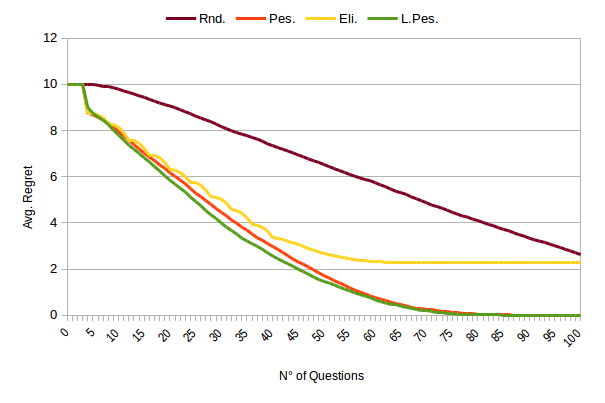
\includegraphics[width=.45\textwidth]{comparison.png}
%\end{figure}
\sisetup{table-number-alignment = center, table-figures-integer=2, table-figures-decimal=1, table-auto-round}
\begin{table}
	\caption{Average MMR in problems of size $(10, 20)$ and geometric weights after $k$ questions.}
	\label{tab:geometricWeights}
	\begin{tabular}{S[table-figures-integer=3, table-figures-decimal=0]S[table-number-alignment = right]@{ ± }S[table-number-alignment = left, table-figures-integer=1]S[table-number-alignment = right]@{ ± }S[table-number-alignment = left, table-figures-integer=1]}
		\toprule
		{k} & {Pes.} & {sd} & {Eli.} & {sd} \\
		\midrule
		0	&20.0	&0.0	&20.0	&0.0\\
		50	&15.96	&0.54	&17.26	&0.42\\
		100	&12.48	&0.93	&15.6	&0.43\\
		150	&9.58	&1.37	&13.94	&0.76\\
		200	&7.43	&1.25	&10.95	&1.12\\
		250	&5.26	&1.52	&6.6	&0.79\\
		300	&3.47	&1.32	&6.57	&0.79\\
		\bottomrule
	\end{tabular}
\end{table}
\paragraph{Comparison of strategies}
Our first experiment concerns small size situations.
\Cref{fig:smallSize} compares some of our strategies in the case $m = 5, n = 10$ (variations around this size yield similar conclusions), where the results are averaged over $200$ runs.
%(The figure also displays the performance of the Elitist strategy, to which we will come back.)
We see that asking random questions does not allow to reach a low regret level even after having asked 100 questions, whereas a low regret level ($\MMR$ = 1) is reached by Pessimistic before having asked 60 questions.
We also see that Pessimistic performs slightly better than Extended pessimistic, showing that Pessimistic chooses candidate questions wisely; this is good news since Pessimistic is much faster: it takes on average only $16$s for a complete elicitation session (for $m = 5$, $n = 10$ and $100$ questions), while Extended pessimistic takes $50$s. Although their performance is close, Pessimistic performs systematically better in multiple runs of the experiment.
\Cref{sec:appendix} provides a problem of larger size.

We also compared the Pessimistic strategy against Elitist in a situation specifically tailored to advantage Elitist. For that experiment specifically, instead of drawing the weights of the oracle randomly, we fix it to a “geometric” weight vector, such that $w_r - w_{r + 1} = 2(w_{r + 1} - w_{r + 2})$, for all $r ≤ m - 2$, so as to dramatically increase the importance of the weights associated to the top ranks. Even in that case, we see in \cref{tab:geometricWeights} that Pessimistic performs better than Elitist.

\paragraph{Evaluation of Pessimistic Strategy}
\label{sec:lowRegret}
Our next set of experiments evaluate the Pessimistic strategy in absolute terms. 
We first wonder how many questions should be asked in order to reach a low regret level. We consider a low level to be a tenth of the number of agents: such a regret is equivalent to the difference of score of an alternative $x$ that results from switching from a profile $P$ to a profile $P'$ where ten percent of the agents rank $x$ last instead of first.
The results for various sizes are displayed in \cref{tab:lowRegret}. 

\commentBN{Replace the following paragraph with real stats on the distribution of questions.}
For the experiments we performed, we see that the number of questions required to reach a low regret level grows approximately linearly with the number of agents and grows less fast than the square of the number of alternatives. Averaging these data by category of value for $m$, and assuming no questions get asked to the chair, we see that in order to reach a low regret level, each agent will have to answer $5.6$ questions for $m = 5$, $17.2$ questions for $m = 10$ and $27.1$ questions for $m = 15$. These numbers have to be contrasted with the estimated number of questions required to elicit the full preference of an agent which are $6.6$ for $m=5$, $24.8$ for $m=10$ and $48.4$ for $m=15$. To obtain these data, we constrained the Pessimistic strategy to ask questions to the agents only, and ran it on a single agent problem, with various values for $m$.

\begin{table}[ht]
	\caption{Number of questions needed by Pessimistic strategy to reach an MMR of $\frac{n}{10}$ (represented by $k_{\MMR}$), by size.}
	\label{tab:lowRegret}
	\begin{tabular}{S[table-figures-decimal=0]S[table-figures-decimal=0]SS[table-figures-integer=3, table-figures-decimal=0]}
		\toprule
		{m} & {n} & {$\frac{n}{10}$} & {$k_{\MMR}$} \\
		\midrule
		5 & 10 & 1 & 60 \\
		5 & 15 & 1.5 & 80 \\
		5 & 20 & 2 & 110 \\
		10 & 20 & 2 & 340 \\
		10 & 30 & 3 & 527 \\
		15 & 30 & 3 & 951 \\
		\bottomrule
	\end{tabular}
\end{table}

%\begin{table}
%	\caption{Number of questions needed by the Pessimistic strategy to elicit the complete preference of one agent.}
%	\label{tab:fullProfile}
%	\begin{tabular}{S[table-figures-decimal=0]S}
%		\toprule
%		{m} & {k} \\
%		\midrule
%		5 & 6.6\\
%		10 & 24.8\\
%		15 & 48.4\\
%		\bottomrule
%	\end{tabular}
%\end{table}

\begin{figure}
	\caption{Average MMR (normalized by $n$) after $k$ questions with Pessimistic strategy for different data sets.}
	\label{fig:linearity}
	\begin{tikzpicture}
		\pgfplotsset{
			every axis legend/.append style={
				at={(0.5,1.1)},
				anchor=south
			},
		}
		\begin{axis}[
			y=80,
			legend columns=3,
			xlabel=Number of Questions,
			ylabel=MMR/n,
			ytick={0,0.5,1},
			xtick distance=100,
			xtick pos=left,
			ymajorgrids=true,
			ytick style={draw=none},
			ymin=0,
			ymax=1,
			xmin=0,
			xmax=1000,
			yticklabels={0,0.5,1},
			legend style={font=\scriptsize}]
			
			\addlegendimage{mark=triangle*,teal,mark size=2}
%			\addlegendimage{mark=*,violet,mark size=2}
			\addlegendimage{mark=square*,green,mark size=2}
			\addlegendimage{mark=diamond*,red,mark size=2}
			\addlegendimage{mark=pentagon*,cyan,mark size=2}
			\addlegendimage{mark=halfcircle*,violet,mark size=2}
			\addlegendimage{mark=*,pink,mark size=2}
			\addlegendimage{mark=halfsquare left*,blue,mark size=2}
			\addlegendimage{mark=halfsquare right*,brown,mark size=2}
			\addlegendimage{mark=halfsquare*,magenta,mark size=2}
			
			
			\addplot[thick, mark=triangle*, mark size = {2}, mark indices = {35}, teal] table [x=k, y=5.10]{data/normalizedLin.dat};
			\addlegendentry{m=5, n=10}
%			\addplot[thick, mark=*, mark size = {2}, mark indices = {45}, violet] table [x=k, y=5.15]{data/normalizedLin.dat};
%			\addlegendentry{m=5, n=15}
			\addplot[thick, mark=square*, mark size = {2}, mark indices = {90}, green] table [x=k, y=5.20]{data/normalizedLin.dat};
			\addlegendentry{m=5, n=20}
			\addplot[thick, mark=diamond*, mark size = {2}, mark indices = {150}, red] table [x=k, y=10.20]{data/normalizedLin.dat};
			\addlegendentry{m=10, n=20}
			\addplot[thick, mark=pentagon*, mark size = {2}, mark indices = {300}, cyan] table [x=k, y=10.30]{data/normalizedLin.dat};
			\addlegendentry{m=10, n=30}
			\addplot[thick, mark=halfcircle*, mark size = {2}, mark indices = {400}, violet] table [x=k, y=tshirt]{data/normalizedLin.dat};
			\addlegendentry{tshirts m11n30}
			\addplot[thick, mark=*, mark size = {2}, mark indices = {400}, pink] table [x=k, y=courses]{data/normalizedLin.dat};
			\addlegendentry{courses m9n146}
			\addplot[thick, mark=halfsquare left*, mark size = {2}, mark indices = {200}, blue] table [x=k, y=14.9]{data/normalizedLin.dat};
			\addlegendentry{m=14, n=9}
			\addplot[thick, mark=halfsquare right*, mark size = {2}, mark indices = {60}, brown] table [x=k, y=skate]{data/normalizedLin.dat};
			\addlegendentry{skate m14n9}
			\addplot[thick, mark=halfsquare*, mark size = {2}, mark indices = {400}, magenta] table [x=k, y=15.30]{data/normalizedLin.dat};
			\addlegendentry{m=15, n=30}
		\end{axis}
	\end{tikzpicture}
\end{figure}

%We next wonder how fast the regret decreases, measured as a function of the number of questions asked. This is important practically because it may be impossible or undesirable to ask sufficient questions to reach a low regret level.
%%Knowing the speed of decrease permits to know which trade-offs can be achieved between the quality of the resulting recommendation and the number of questions that participants have to answer. 
%\Cref{fig:linearity} shows graphically the decrease in MMR according to the number of questions asked for various problem sizes. We see that this function is convex, apart from the very first few questions, indicating %to users of our approach 
%that, on average, halving the number of questions will only reduce the gain in regret by less than half. %\commentBN{Reviewer: Halving the number of questions reduces the regret by more than 50\%.}
%At the start of the elicitation, the space of uncertainty is so large that the adversary can attain the maximum possible value of regret; multiple answers are needed to constrain her enough for the MMR to start decreasing. When approaching optimality, the pace of MMR reduction decreases.

In \cref{fig:linearity} we can also observe, as expected, that given a problem size the number of questions needed to reach a given MMR is lower when considering a real data set than a IC generated profile. \commentBN{Add the following:}
By looking at the data we observe that:
\begin{itemize}
	\item \textit{Skate} - the top-2 alternatives are the same for all voters, and 8 out of 9 voters rank the same alternative at position 3;
	\item \textit{AGH} - all voters rank the same alternative at the top position, different group of voters share the same preference rankings;
	\item \textit{T Shirt} - the alternatives are evenly distributed in the preference rankings.
\end{itemize}
The experiments suggest that high degree of similarity in the preference rankings helps reducing the regret faster.
% do less harm than halving the gain in regret, on average.

%\subsection{Value of information comparison}
\paragraph{Comparison with Two Phase}
\begin{table}
	\caption{Average MMR in problems of size $(10, 20)$ after $400$ questions, among which $q_c$ to the chair.}
	\label{tab:twoP400}
	\begin{tabular}{S[table-figures-integer=3, table-figures-decimal=0]S[table-number-alignment = right]@{ ± }S[table-number-alignment = left, table-figures-integer=1]S[table-number-alignment = right]@{ ± }S[table-number-alignment = left, table-figures-integer=1]}
		\toprule
		{$q_c$} & {2 ph.\ ca} & {sd} & {2 ph.\ ac} & {sd} \\
		\midrule
		0 & 0.66 & 0.67 & 0.65 & 0.65  \\
		15 & 0.71 & 0.73 & 0.67	& 0.64 \\
		30 & 0.62 & 0.5 & 0.8 & 0.62 \\
		50 & 1.23 & 1.46 & 0.8 & 0.79 \\
		100 & 2.03 & 1.56 & 1.88 & 1.02  \\
%		150 & 3.41 & 1.79 & 4.07 & 1.51 \\
		200 & 4.61	& 1.35  & 6.53 & 2.0  \\
%		250 & 8.4 & 1.86 & 	7.69 & 1.24 \\
		300 &11.07 & 0.86& 11.87 & 1.25 \\
%		350 &15.06 & 0.68&15.59 & 0.6 \\
		400 &20.0 & 0.0 & 20.0 & 0.0 \\
		\bottomrule
	\end{tabular}
\end{table}

The experiments so far let the strategy target its questions unrestrictively, leaving open the possibility of questioning either the chair or an agent at each step. One may wonder what is lost in terms of regret by asking different proportions of questions to the chair and the agents. Such restrictions may be useful because of (partial) unavailability of the chair, or because the estimated cognitive costs may differ sensibly, as these types of questions differ in nature. 
\Cref{tab:twoP400} shows the MMR value reached in problems of size $m = 10, n = 20$ after $400$ questions, using the Two phases strategy, in the “ca” (chair then agents) and in the “ac” (agents then chair) variants. These numbers are to be compared with the MMR value reached after 400 questions with the Pessimistic strategy (displayed in \cref{fig:linearity}), which is $0.6$.
The Pessimistic strategy asks on average $48$ questions to the chair in this setting.

These numbers highlight that it is possible to obtain a good-quality recommendation while knowing only that the voting rule is a scoring rule and that the weights are convex, which is our basic hypothesis (corresponding to the line $q_c = 0$, where no question is asked to the chair).

\section{Conclusions}  
\label{sec:conclusions}
In this paper we have considered a social choice setting with partial information about the agent's preferences and a partially specified voting rule.
In this setting, we have proposed the use of minimax regret both as a means of robust winner determination as well as a guide to the process of simultaneous elicitation of preferences and voting rule.
Our experimental results %on randomly generated and real world data sets 
suggest that regret-based elicitation is effective and allows to quickly reduce worst-case regret significantly. They also show that, in our setting, good quality (low regret) recommendations can be achieved short of knowing the weights precisely or the profile completely.
%regret, but they also show that starting with zero knowledge became a pretentious approach really quickly when increasing the size of the problem. Future works will therefore include the test of these strategies on partial specified profiles, ideally on real datasets. An other important direction is the extension to voting rules beyond scoring rules.
%Regret-based elicitation allows to determine near-optimal winners using only few information about the agent preferences.

As part of our contribution, a general open-source library, allowing to reproduce our experiments and perform many more, will be made publicly available (URL not displayed for ensuring anonymity).
%and serve as a basis for further research

%We mention some directions for future works.
Further development of elicitation strategies, considering alternative heuristics, is an important direction. 
Second, elicitation could be extended to voting rules beyond scoring rules. 
Finally, an important direction of extension aims at studying how to elicit preferences while restraining to concrete and easy questions.
% Acknowledgments: We thank the reviewers for comments helping to improve the paper. 

%%%%%%%%%%%%%%%%%%%%%%%%%%%%%%%%%%%%%%%%%%%%%%%%%%%%%%%%%%%%%%%%%%%%%%%%

%%% The acknowledgments section is defined using the "acks" environment
%%% (rather than an unnumbered section). The use of this environment 
%%% ensures the proper identification of the section in the article 
%%% metadata as well as the consistent spelling of the heading.

%\begin{acks}
%If you wish to include any acknowledgments in your paper (e.g., to 
%people or funding agencies), please do so using the `\texttt{acks}' 
%environment. Note that the text of your acknowledgments will be omitted
%if you compile your document with the `\texttt{anonymous}' option.
%\end{acks}

%%%%%%%%%%%%%%%%%%%%%%%%%%%%%%%%%%%%%%%%%%%%%%%%%%%%%%%%%%%%%%%%%%%%%%%%

%%% The next two lines define, first, the bibliography style to be 
%%% applied, and, second, the bibliography file to be used.
%\bibliographystyle{abbrvnat} 
%\bibliography{biblio}

\newpage
\bibliographystyle{named}
{\small \bibliography{biblio}}

\newpage
\appendix
\section{Appendix}
\label{sec:appendix}
\newtheorem*{details*}{Strategy Details}

\begin{details*}[Pessimistic]
	Given $j \in N^*$, if $x^*$ and $\bar{y}$ are incomparable in $\ppref_j$, the candidate question concerns the pair $(x^*, \bar{y})$, otherwise, the candidate question concerns the pair $(x^*, z)$ for some $z$ incomparable to $x^*$ (randomly chosen), or if none such $z$ exist, the pair $(\bar{y}, z)$ for some $z$ incomparable to $\bar{y}$, or, if both $x^*$ and $\bar{y}$ are comparable to every alternatives in $\ppref_j$, any incomparable pair is picked at random. 
%Responses to questions involving $x^*$ or $\bar{y}$ constrain the ability of the adversary to complete the profile in such manner, possibly reducing minimax regret.
	Once having selected $n + m$ candidate questions, the Pessimistic strategy selects the one that leads to minimal regret in the worst case, considering both possible answers to the question, and with penalty terms depending on the kind of question. To define this comparison precisely, assume that a question $q_1$ has type $t_1$ (being “chair” or “agent”), and leads to the new knowledge states $(\pprofile_1, W_1)$ if answered positively and $(\pprofile'_1, W'_1)$ if the answer is negative. 
	Define $R^{\max}_1 = \max\set{\MMR(\pprofile_1, W_1), \MMR(\pprofile'_1, W'_1)}$
	and $R^{\min}_1 = \min\set{\MMR(\pprofile_1, W_1), \MMR(\pprofile'_1, W'_1)} \epsilon_{t} + \epsilon'_{t}$.
	%If $(\pprofile_1, W_1) ≥ (\pprofile'_1, W'_1)$, define $\MMR^{\max} = \MMR(\pprofile_1, W_1)$ and $\MMR^{\min} = \MMR(\pprofile'_1, W'_1)$; otherwise, define $\MMR^{\max} = \MMR(\pprofile'_1, W'_1)$ and $\MMR^{\min} = \MMR(\pprofile_1, W_1)$.
	% and and $(\pprofile^\min_2, W^\min_2)$. numbering them so that $\MMR(\pprofile_1, W_1) ≥ \MMR(\pprofile_2, W_2)$. Then the badness of the question in the worst case is:
	The terms $\epsilon_t$ and $\epsilon'_{t}$ are real numbers associated to the type $t$ of question; these parameters are to be determined experimentally and are used to fine control the choice of the question type.
	Define similarly $t_2$, $R^{\max}_2$ and $R^{\min}_2$ for a question $q_2$.
	We are now faced with the problem of aggregating these values in order to compare the informative values of the candidate questions. We adopt a pessimistic approach, reported to perform better than optimistic aggregation \citep{Cailloux2014}, although our experiments in this context suggested a weak impact of that choice on the performance of the strategy.
	To avoid the absorption property of the max, we adopt $\leximax$ as an aggregator.
	Pessimistic thus considers question $q_1$ to be better  than $q_2$ iff $R^{\max}_1 < R^{\max}_2 \text{ or } [R^{\max}_1 = R^{\max}_2 \text{ and } R^{\min}_1 < R^{\min}_2]$.
	%This comparison gives a way of picking questions among a set of possible questions, by picking one that minimizes this approximate measure of minimax regret {\em a posteriori}. 
	%The motivation for using this operator lies in 
	In other words if the maximal {\em a posteriori} MMR of two questions are (nearly) equal, then it considers the (penalized) minimal MMR values, preferring the question with the lowest value.
	(Technically, instead of applying a pure lexicographic aggregation, which is very sensitive to small errors due to floating-point computations, we apply a weighted sum between the maximal and the penalized minimal MMR values, with a predominant weight given to the maximal one, several order of magnitudes higher than the weight given to the penalized minimal MMR.)

The penalty parameters for the Pessimistic and Extended pessimistic strategies are set to $\epsilon_{\text{chair}} = 1.1$, $\epsilon'_{\text{chair}} = 10^{-6}$, $\epsilon_{\text{agent}} = 1.0$ and $\epsilon'_{\text{agent}} = 0$.
\end{details*}

\begin{sketch*}[\cref{claim:completion}]
	Consider our knowledge $\pprefeq_j$ about the preference of the agent $j$. 
	The adversary's goal is to make the score of $y$ as high as possible and the score of $x$ as low as possible. 
	To do this, he should complete $\ppref_j$ to $\pref_j$ by putting above $x$ as many alternatives as he can, that is, all the alternatives except those that are known to be worse than $x$ (those $a$ such that $x \pprefeq_j a$); and similarly, he should put below $y$ all the alternatives he can. Two conditions must be excluded for $a$ to go below $y$. The alternatives such that $a \pprefeq_j y$ can’t be put below $y$.
	Furthermore, the first objective must take priority over the second one: when an alternative should go above $x$ according to the first objective (because $¬(x \pprefeq_j a)$), and $x$ is known to be better than $y$ (thus $x \pprefeq_j y$), then $a$ should be put above $x$ (irrespective of whether $a \pprefeq_j y$), which will move both $x$ and $y$ one rank lower than if $a$ had been put below $y$. 
	This maximizes the adversary’s interests: because the weight vector is convex, the difference of scores will be lower when both alternatives are ranked lower (Equation \ref{eq:convexity}), and that difference of scores is in favor of $x$ when $x \ppref_j y$, thus to be minimized from the point of view of the adversary.
\end{sketch*}

\begin{proof*}[\cref{claim:rankPMR}]
	The rank of $x$ is directly obtained from \cref{eq:complx}. The rank of $y$ is obtained by complementing \cref{eq:comply}, obtaining $a \prefeq_j y ⇔ (a \pprefeq_j y) ∨ ((x \pprefeq_j y) ∧ ¬(x \pprefeq_j a))$, and, observing that $a \pref_j y ⇔ a ≠ y ∧ a \prefeq_j y$, obtaining that $a \pref_j y$ if and only if
	\begin{equation}
		\label{eq:betteryinter}
		(a \neq y) ∧ [(a \pprefeq_j y) ∨ ((x \pprefeq_j y) ∧ ¬(x \pprefeq_j a))],
	\end{equation} 
	or equivalently, if and only if
	\begin{equation}
		\label{eq:bettery}
		%a \pref_j y ⇔ 
		(a \ppref_j y) ∨ ((x \pprefeq_j y) ∧ ¬(x \pprefeq_j a)).
	\end{equation} 
	Indeed, \eqref{eq:betteryinter} $⇒$ \eqref{eq:bettery}, and \eqref{eq:bettery} $⇒$ \eqref{eq:betteryinter} because $(x \pprefeq_j y) ∧ ¬(x \pprefeq_j a) ⇒ a ≠ y$ (as when $a = y$, $(x \pprefeq_j y)$ and $¬(x \pprefeq_j a)$ are opposite claims). Suffices now to rewrite \cref{eq:bettery} to let the two disjuncts designate disjoint sets:
	\begin{equation}
		\label{eq:betteryfinal}
		a \pref_j y ⇔ 
		(a \ppref_j y) ∨ ((x \pprefeq_j y) ∧ ¬(x \pprefeq_j a) ∧ ¬(a \ppref_j y)).
	\end{equation}
\end{proof*}

\begin{proof*}[\cref{prop:chairQuestions}]
	\label{proof:chairQuestions}
	Define a linear order $>_1$ over $A$ as placing $a$ at rank $r$, $b$ at rank $r + 1$, and the remaining alternatives arbitrarily. 
	Define a linear order $>_2$ over $A$ as placing $a$ at rank $r + 2$, $b$ at rank $r + 1$, and the remaining alternatives arbitrarily.
	Define an arbitrary linear ordering $>$ over $A \setminus \set{a, b}$. 
	Define a linear order $>_3$ as placing $a$ first, $b$ second, and following the order of $>$ for the remaining positions.
	Finally, define a linear order $>_4$ as placing $b$ first, $a$ second, and following the \emph{inverse} order of $>$ for the remaining positions.
	
	Define $P$ as the profile of $3 (p + q)$ voters containing $q$ times $>_1$, $p$ times $>_2$, and $>_3$ and $>_4$ each $p + q$ times.
	As a result, $a$ obtains the following ranks: $q$ times $r$, $p$ times $r + 2$, $p + q$ times first, and $p + q$ times second. The alternative $b$ obtains the ranks $r + 1$, $2$ and $1$, each $p + q$ times. Consider any alternative $c \in A \setminus \set{a, b}$. Its score is maximal when it comes first in $>_1$, first in $>_2$ and first in $>$, by convexity of the weights. In that case, $c$ is positioned at the ranks $1$, $3$ and $m$, each $p + q$ times. 
	
	Letting $s(x)$ denote the score of $x$ at $P$, we obtain $s(a) = q w_r + p w_{r + 2} + (p + q) w_1 + (p + q) w_2$, thus, $s(a) ≥ (p + q) w_m + (p + q) w_1 + (p + q) w_2$; $s(b) = (p + q) w_{r + 1} + (p + q) w_2 + (p + q) w_1$; and, $\forall c \in A \setminus \set{a, b}$, 
	$s(c) ≤ (p + q) w_1 + (p + q) w_3 + (p + q) w_m$. It follows that $a$ or $b$ maximize $s$ (as $s(a) ≥ s(c)$). We conclude by observing that $a \in f(P) ⇔ s(a) ≥ s(b) ⇔ q w_r + p w_{r + 2} ≥ (p + q) w_{r + 1} ⇔ w_r - w_{r + 1} ≥ (p / q) (w_{r + 1} - w_{r + 2})$, and similarly for $b \in f(P)$.
\end{proof*}

\sisetup{table-number-alignment = center, table-figures-integer=2, table-figures-decimal=1, table-auto-round}
\begin{table}[ht]
	\caption{Average MMR in problems of size $(10, 20)$ after $k$ questions.}
	\label{tab:biggerSize}
	\begin{tabular}{S[table-figures-integer=3, table-figures-decimal=0]S[table-number-alignment = right]@{ ± }S[table-number-alignment = left, table-figures-integer=1]S[table-number-alignment = right]@{ ± }S[table-number-alignment = left, table-figures-integer=1]S[table-number-alignment = right]@{ ± }S[table-number-alignment = left, table-figures-integer=1]S[table-number-alignment = right]@{ ± }S[table-number-alignment = left]}
		\toprule
		{k} & {Rnd.} & {sd} & {Pes.} & {sd} & {Eli.} & {sd} \\
		\midrule
		0 &20.0 & 0.0 & 20.0 & 0.0&  20.0 & 0.0 \\
		50 & 19.82 & 0.04 &	15.59 &0.56	&17.38& 0.7\\
		100 & 19.12	& 0.26&	11.91&	1.26 &15.23& 0.73\\
		150 & 18.06	& 0.47&	8.92&	1.53 &13.38& 1.11\\
		200 & 16.89	& 0.62&6.24&2.02&11.76& 1.03\\
		250 & 15.63 & 0.84&	4.64&1.72&10.56& 0.89\\
		300 & 14.72	& 0.94&	3.01& 1.35 &10.48& 0.87\\
		350 & 13.41	& 1.15& 1.76& 0.95&10.48& 0.86\\
		400 & 11.98	& 0.68&	0.62&0.56 &10.48& 0.86\\
		\bottomrule
	\end{tabular}
\end{table}
\Cref{tab:biggerSize} shows that the conclusions of \cref{fig:smallSize} also hold for a problem of larger size ($m = 10, n = 20$), except that this table does not feature Extended pessimistic, which is too slow to be run repeatedly on such instance.






\end{document}

%%%%%%%%%%%%%%%%%%%%%%%%%%%%%%%%%%%%%%%%%%%%%%%%%%%%%%%%%%%%%%%%%%%%%%%%




%%%%%%%%%%%%%%%%%%%%%%%%%%%%%%%%%%%%%%%%%%%%%%%%%%%%%%%%%%%%%%%%%%%%%%%%



